\section{Theoretische Grundlagen}
\label{sec:theorie}
In diesem Versuch soll aus der Untersuchung der Molwärme $C_V$
die materialspezifische Debye-Temperatur $\theta_\text{D}$ von Kupfer
bestimmt werden.
Während eine klassische Betrachtung eine konstanten Wert für $C_V$
liefert, erhält man mit Einbeziehung quantenmechanischer Effekte eine
Temperaturabhängigkeit, die im Folgenden beschrieben und schließlich 
gemessen wird.

\subsection{Klassiche Theorie der Molwärme}
\label{subsec:klassisch}
In der klassischen Wärmelehre verteilt sich die Energie in einem Körper
gleichmäßig auf alle Atome. Dabei entfallen auf jeden Freiheitsgrad im Mittel
der Anteil $\sfrac{1}{2}\kb T$, mit der Boltzmannkonstante $\kb$ und der
Temperatur $T$.
In einem Festkörper sitzen die Atome an festen Gitterplätzen, um die sie
Schwingungen in alle Raumrichtungen ausführen können. Für einen harmonischen
Oszillator entspricht die mittlere kinetische Energie der mittleren
potentiellen Energie, weshalb die gesamte Energie $U$ eines Mols klassisch
durch
\begin{equation}
    \label{eqn:innere_energie}
    U = 3 \kb \mathup{N}_\text{A} T = 3\mathup{R}T
\end{equation}
gegeben ist. Hierbei bezeichnet $\mathup{N}_\text{A}$ die Avogadrokonstante
und $\mathup{R}$ die allgemeine Gaskonstante.

Die Spezifische Molwärme ist durch die Ableitung der inneren Energie $U$ nach
der Temperatur bei konstantem Volumen definiert. Es folgt damit
die bekannte, temperatur- und materialunabhängige Größe
\begin{equation}
    \label{eqn:cv_klassisch}
    C_V = \left.\frac{\partial U}{\partial T}\right|_V = 3 \mathup{R}\,.
\end{equation}

\subsection{Das Einstein-Modell}
\label{subsec:einstein}
Für gebräuchliche Temperaturen von $T \approx \SI{300}{\kelvin}$ und mehr
stimmt die klassische Betrachtung gut mit Messungen überein.
Bei tieferen Temperaturen wird die Molwärme von Stoffen jedoch
temperaturabhängig.
Das Einstein-Modell erweitert die klassische Betrachtung deshalb um die
Quanteneigenschaften der Atome. Dazu fordert es, dass die Energieüberträge
der Oszillatoren ein ganzzahliges Vielfaches von $\hbar\omega$ -- mit
der Kreisfrequenz $\omega$ der schwingenden Atome und dem reduziertem Plankschem Wirkungsquantum $\hbar$ -- betragen müssen.
Die Besetzung der Energiezustände $n = 0,1,2,\dots$ ist dann Boltzmann-verteilt
und es gilt für die Wahrscheinlichkeit $W$, dass ein solcher Zustand besetzt
ist:
\begin{equation}
    \label{eqn:boltzmann}
    W(n) = \exp\left[-\frac{n\hbar\omega}{\kb T}\right]\,.
\end{equation}
Durch Summation und Normierung über alle möglichen Zustände eines Atoms
lässt sich dann die mittlere Energie dieses Atoms bestimmen zu
\begin{equation}
    \label{eqn:u_einstein}
    \left<u\right>_\text{Einstein} =
    \frac{\hbar\omega}{\exp[\frac{\hbar\omega}{\kb T}] - 1}\,.
\end{equation}
Daraus folgt die Molwärme im Einstein-Modell:
\begin{equation}
    \label{eqn:cv_einstein}
    C_{V,\text{Einstein}} =
    3\mathup{R}\left(\frac{\hbar\omega}{\kb T}\right)^2
    \frac{
        \exp[\frac{\hbar\omega}{\kb T}]
    }{
        \left(\exp[\frac{\hbar\omega}{\kb T}] - 1\right)^2
    }\,,
\end{equation}
was im Limes für große Temperaturen gegen den klassischen Wert
$C_V = 3\mathup{R}$ strebt.
Diese Form beschreibt die Temperaturabhängigkeit der Molwärme besser als
die klassische Annahme. Weil jedoch die Kreisfrequenzen der Atome im Festkörper
nicht homogen verteilt sind, beinhaltet diese Betrachtung noch immer eine grobe
Näherung.

\subsection{Das Debye-Modell}
\label{subsec:debye}
Das oben beschriebene Einstein-Modell wird im Debye-Modell um eine spektrale
Verteilung $Z(\omega)$ der Frequenzen aller Oszillatoren des Kristalls
ergänzt.
Unter der Annahme eines isotropen und dispersionsfreien Mediums lässt sich
$Z(\omega)$ durch Abzählen aller Eigenschwingungen in einem Würfel
der Kantenlänge $L$ im Frequenzintervall von $\omega$ bis
$\omega+\mathup{d}\omega$ bestimmen:
\begin{equation}
    \label{eqn:z}
    Z(\omega)\mathup{d}\omega = \frac{3L^3}{2\pi^2 v^3} \mathup{d}\omega\,,
\end{equation}
wobei $v$ die Phasengeschwindigkeit im Kristall bezeichnet.
Über die Anzahl $3N$ der Eigenschwingungen eines Kristalls aus $N$ Atomen
lässt sich eine obere Grenzfrequenz -- die Debye-Frequenz -- bestimmen zu
\begin{equation}
    \label{eqn:omega_debye}
    \omega_D^3 = \frac{6\pi^2 v^3 N}{L^3} = \frac{18 \pi^2 N}{L^3} \frac{1}{\frac{1}{v_\text{l}^3}+\frac{2}{v_\text{tr}^3}},.
\end{equation}
Mit den Abkürzungen $x = \hbar\omega/\kb T$ und der Debye-Temperatur
$\theta_\text{D}$ mit $\theta_\text{D}/T = \hbar\omega_D/\kb T$ folgt
für die Molwärme im Debye-Modell
\begin{equation}
    \label{eqn:cv_debye}
    C_{V,\text{Debye}} =
    9\mathup{R}\left(\frac{T}{\theta_\text{D}}\right)^3
    \int_0^{\frac{\theta_\text{D}}{T}}
    \frac{x^4\e^x}{\left(\e^x-1\right)^2}\mathup{d}x\,.
\end{equation}
Die Debye-Temperatur stellt eine Materialkonstante dar und entspricht der
Größenordnung, ab derer ein klassisches Verhalten der Molwärme eintritt.
Die Funktion $C_V = f(\theta_\text{D}/T)$ beschreibt dann einen universellen
Zusammenhang. Für hohe Temperaturen $x \ll \num{1}$ zeigt auch sie das
asymptotische Verhalten $C_V\to 3\mathup{R}$.
Bei tiefen Temperaturen liefert das Debye-Modell jedoch eine wesentlich
bessere Näherung, als das Einstein-Modell.
Für eine Exakte Beschreibung der Molwärme müsste schließlich die Dispersion,
sowie der Beitrag der Leitungselektronen im Kristall betrachtet werden.
Für diesen Versuch ist die Nutzung des Debye-Modells dennoch ausreichend.

\section{Durchführung}
\label{sec:durchführung}
Um die Debye-Temperatur $\theta_\text{D}$ von Kupfer zu bestimmen, wird
eine Kupferprobe elektrisch von $T \approx \SI{80}{\kelvin}$ auf etwa
$T \approx \SI{300}{\kelvin}$ erwärmt.
Dabei wird die zugeführte Energie, sowie die Temperatur der Probe gemessen,
woraus die Wärmekapazität bei konstantem Druck $C_p$ bestimmt werden kann.
Der Zusammenhang zur Molwärme $C_V$ lautet:
\begin{equation}
    \label{eqn:cp_cv}
    C_p - C_V = 9\alpha^2\kappa V_0 T\,
\end{equation}
mit dem linearen Ausdehnungskoeffizienten $\alpha$, dem Kompressionsmodul
$\kappa$ und dem Molvolumen $V_0$.

Die Probe befindet sich in einem Gehäuse, welches in einem Dewargefäß
mit flüssigem Stickstoff auf etwa $T=\SI{80}{\kelvin}$ gekühlt wird.
Das Gehäuse wird zuerst mit Helium geflutet und evakuiert, sobald sich
Gehäuse- und Probentemperatur angeglichen haben.
Durch das Vakuum ist die Probe thermisch isoliert.
Erwärmung oder Abkühlen durch Wärmestrahlung wird mit Hilfe einer Heizung
im Gehäuse verhindert, welche den Temperaturunterschied zwischen diesem und
der Probe möglichst gering halten soll.
Abbildung \ref{fig:aufbau} skizziert den Versuchsaufbau.
Die Temperatur von Gehäuse und Probe wird jeweils mit einem Ohmschen Widerstand
bestimmt.
Die zugeführte Energie entspricht der elektrischen Leistung über die Zeit
der Probenheizung.
\begin{figure}
    \centering
    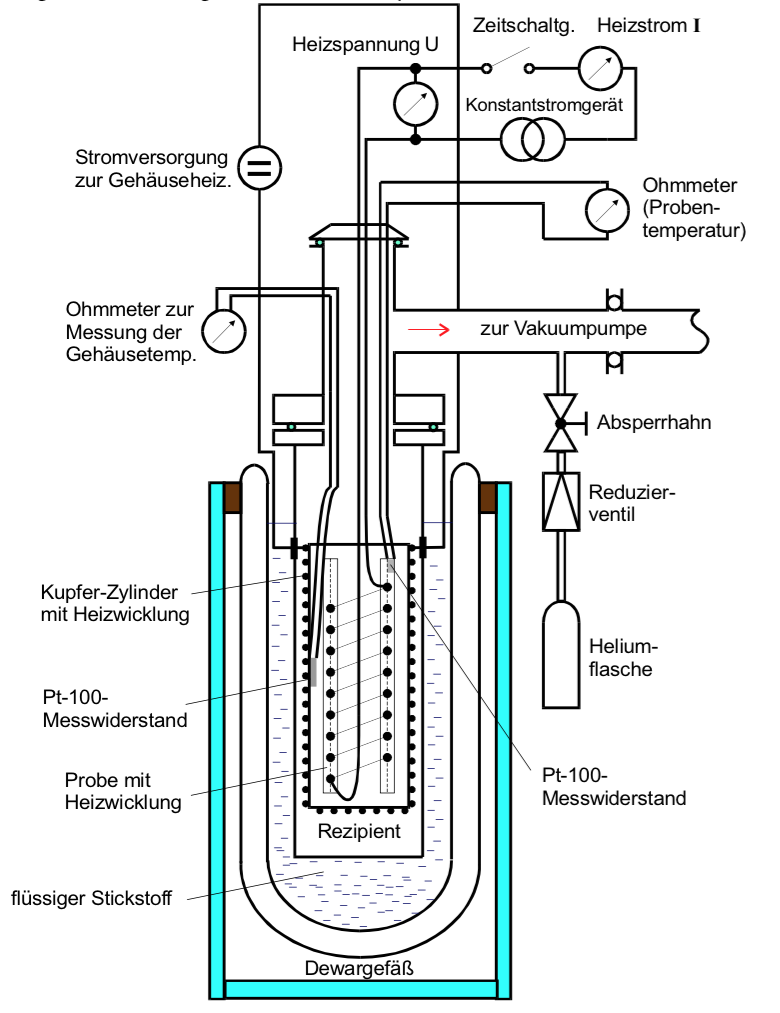
\includegraphics[width=0.6\linewidth]{img/aufbau.png}
    \caption{
        Versuchsaufbau \cite{V47}, bestehend aus Dewargefäß, in das ein beheizbares
        Gehäuse mit ebenfalls beheizbarer Probe eingelassen wird.
        Das Gefäß ist mit flüssigem Stickstoff befüllt und das Gehäuse
        evakuiert.
    }
    \label{fig:aufbau}
\end{figure}
